\documentclass[a4paper,fleqn]{cas-dc}

% If the frontmatter runs over more than one page
% use the longmktitle option.

%\documentclass[a4paper,fleqn,longmktitle]{cas-dc}

\usepackage[numbers]{natbib}
%\usepackage[authoryear]{natbib}
%\usepackage[authoryear,longnamesfirst]{natbib}

%%%Author macros
\def\tsc#1{\csdef{#1}{\textsc{\lowercase{#1}}\xspace}}
\tsc{WGM}
\tsc{QE}
%%%

% Uncomment and use as if needed
%\newtheorem{theorem}{Theorem}
%\newtheorem{lemma}[theorem]{Lemma}
%\newdefinition{rmk}{Remark}
%\newproof{pf}{Proof}
%\newproof{pot}{Proof of Theorem \ref{thm}}

\begin{document}
\let\WriteBookmarks\relax
\def\floatpagepagefraction{1}
\def\textpagefraction{.001}

% Short title
\shorttitle{Meta--heuristic parameter estimation of solar cells with S--shaped IV characteristics}

% Short author
\shortauthors{O. Olikh}

% Main title of the paper
\title [mode = title]{Estimation of parameters for solar cells with S--shaped current--voltage characteristics using meta--heuristic algorithms}

% First author
%
% Options: Use if required
% eg: \author[1,3]{Author Name}[type=editor,
%       style=chinese,
%       auid=000,
%       bioid=1,
%       prefix=Sir,
%       orcid=0000-0000-0000-0000,
%       facebook=<facebook id>,
%       twitter=<twitter id>,
%       linkedin=<linkedin id>,
%       gplus=<gplus id>]
\author{Oleg~Olikh}
%\cormark[1]
\ead{olegolikh@knu.ua}
%\address[1]{Taras Shevchenko National University of Kyiv, 64/13, Volodymyrska Street, City of Kyiv, Ukraine, 01601}


% Address/affiliation
\affiliation{organization={Taras Shevchenko National University of Kyiv},
            addressline={64/13, Volodymyrska Street},
            city={Kyiv},
%          citysep={}, % Uncomment if no comma needed between city and postcode
            postcode={01601},
 %           state={},
            country={Ukraine}}

% For a title note without a number/mark
%\nonumnote{}

% Here goes the abstract
\begin{abstract}
Defect-assisted recombination processes frequently
limit the photovoltaic device performance.
The low-cost and express methods of impurity contamination control
are in demand at solar cell manufacturing.
In this paper, we applied deep learning-based
approach to extract the iron concentration in silicon solar cell from an
ideality factor values.
\end{abstract}

% Use if graphical abstract is present
%\begin{graphicalabstract}
%\includegraphics{}
%\end{graphicalabstract}

% Research highlights
\begin{highlights}
\item Proposed deep learning-based method to predict iron contamination in Si-SC by using IV curve.
\item The simulated IV characteristics are used to create training and test datasets.
\item The DNN's configurations are proposed.
\item The mean squared relative error of prediction is up to 0.005.
\end{highlights}

% Keywords
% Each keyword is seperated by \sep
\begin{keywords}
Ideality factor \sep Silicon \sep $n^+$--$p$--$p^+$ structure \sep
SCAPS \sep Iron contamination \sep Machine learning
\end{keywords}

\maketitle

% Main text
\section{Introduction}\label{Int}

\section{Models and Methods}\label{MM}
\subsection{Solar cell model}\label{SCModel}
Fig.~\ref{fig_chem}
vividly reveals the structure of the used model \cite{Castro2010}.
It can be seen from the figure that model contains a current source accompanied by a diode D1, a shunt
resistor $R_\mathrm{p1}$ to show the leakage current, and a series resistor $R_\mathrm{s}$ to consider the
losses associated with the load current.
Besides, the second diode D2 with a second parallel resistance $R_\mathrm{p2}$ is placed opposite to the first one and is essential to
simulate the non-ideal effects of the active layer/cathode interface.
In this model, D1 is responsible for the exponential behavior of the I--V curve,
the main contribution of D2 is to simulate the S--shape.
The analytical solution $V(I)$ of the opposed two--diode equivalent circuit model was
 obtained \cite{CastroSolution} using Lambert $W$-function \cite{LambertNew}:


\begin{figure}[]
	\centering
		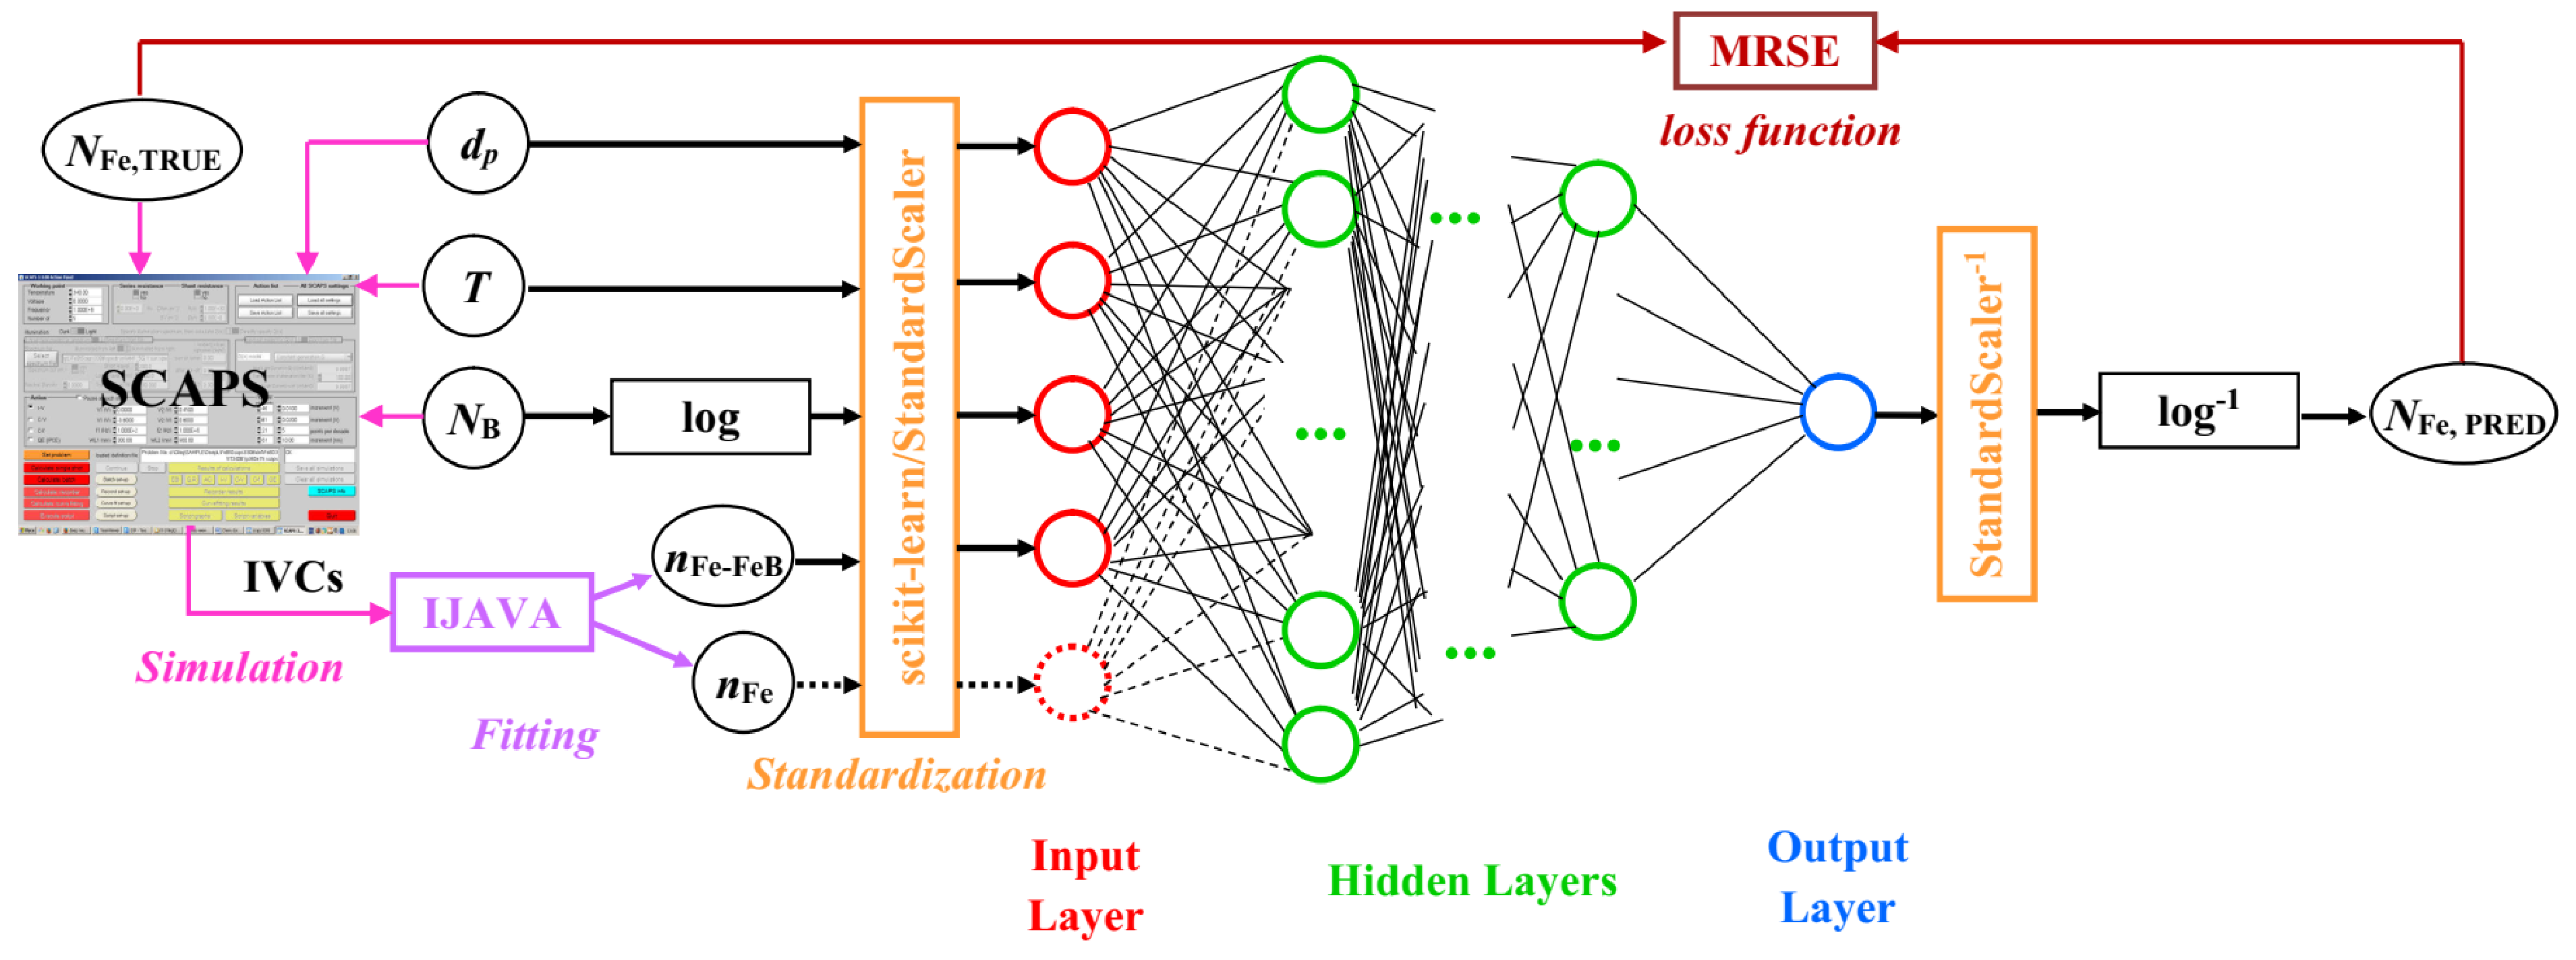
\includegraphics[width=0.9\columnwidth]{Chem}
	  \caption{The opposed two--diode equivalent--circuit model of a solar cell.}\label{fig_chem}
\end{figure}


\begin{eqnarray}
% \nonumber to remove numbering (before each equation)
\label{eqIV_W}
V&=& (I+I_\mathrm{ph}+I_{01})R_\mathrm{p1} \nonumber \\
  &&-\frac{n_1kT}{q}W\left\{\frac{qI_{01}R_\mathrm{p1}}{n_1kT}\exp\left[\frac{qR_\mathrm{p1}(I+I_\mathrm{ph}+I_{01})}{n_1kT}\right]\right\} \nonumber \\
  &&+\frac{n_2kT}{q}W\left\{\frac{qI_{02}R_\mathrm{p2}}{n_2kT}\exp\left[-\frac{qR_\mathrm{p2}(I-I_{02})}{n_2kT}\right]\right\} \nonumber \\
  &&+(I-I_{02})R_\mathrm{p2}+IR_\mathrm{s}\,,
\end{eqnarray}
where
$I_{01}$ and $I_{02}$ are the saturation currents and
$n_1$ and $n_2$ are
the ideality factors for D1 and D2 respectively,
and $I_\mathrm{ph}$ is the ideal photocurrent.
Thus, the model employs eight lumped parameters
($I_{01}$, $n_1$, $R_\mathrm{p1}$, $I_{02}$, $n_2$, $R_\mathrm{p2}$,
$R_\mathrm{s}$, and $I_\mathrm{ph}$)
that need to be determined from the I-V curve.
Thus, from an optimization perspective, the dimension of the problem is $D=8$.

The expression~(\ref{eqIV_W}) has a drawback in that it tends to stray from the range of numbers that can be accommodated by the standard 64-bit floating-point format owing to the presence of exponential functions for larger numbers.
To overcome this drawback, the use of the $g$--function $g(x)=\ln(W(\exp(x)))$ was suggested \cite{roberts2015calculating}.
The analytical solution $V(I)$ using the $g$--function is as follows \cite{roberts2015calculating}
\begin{equation}
\label{eqIV_g}
\begin{split}
V(I)= &IR_\mathrm{s}+\frac{n_1kT}{q}g(x_1)-\frac{n_2kT}{q}g(x_2) \\
  &-\frac{n_1kT}{q}\ln\left[\frac{qI_{01}R_\mathrm{p1}}{n_1kT}\right] +\frac{n_2kT}{q}\ln\left[\frac{qI_{02}R_\mathrm{p2}}{n_2kT}\right]\,,
\end{split}
\end{equation}
with
\begin{equation}
\label{eqx1}
x_1= \ln\left(\frac{qI_{01}R_\mathrm{p1}}{n_1kT}\right)+\frac{q(I+I_\mathrm{ph}+I_{01})R_\mathrm{p1}}{n_1kT}\,,
\end{equation}
and
\begin{equation}
\label{eqx2}
x_2= \ln\left(\frac{qI_{02}R_\mathrm{p2}}{n_2kT}\right)-\frac{q(I-I_{02})R_\mathrm{p2}}{n_2kT}\,.
\end{equation}
We used Eqs.~(\ref{eqIV_g})--(\ref{eqx2}) both for simulation I--V curves and during the approximation procedure.
The $g$--function was evaluated by using iterative procedure \cite{roberts2015calculating}.

\subsection{Meta-heuristic algorithms}\label{MHA}
In the literature, meta-heuristics are frequently categorized based on their sources of inspiration.
This categorization involves incorporating elements of true simulations and principles that incorporate stochasticity,
with the objective of emulating diverse characteristics observed in biological behavior, the lives of creatures in nature, human behavior, or natural phenomena.
On this basis, any meta-heuristic algorithm can fall into one of the following main classes \cite{WhiteShark,Gannet,Dandelion}:
evolution-based methods (emulate the principles of evolutionary behavior observed in creatures in nature by relying on the concept of survival of the fittest),
swarm intelligence--based methods (simulate the collective, dynamic, intelligent, and concerted gregarious conduct of collections of flocks or communities found in nature),
bio--based methods (use biological processes unrelated to group behavior),
chemical \& physical--based methods (originate from the physical phenomena or chemical laws that exist in the universe),
human-society--based methods (inspired by human beings, including various activities such as thinking and social behavior),
and math--based methods (borrow the mathematical functions).
Generally, there are hundreds of meta-heuristic optimization methods available.
While we acknowledge that our selection may not be fully comprehensive,  
we utilized 14 methods, representing all classes mentioned above, 
to tackle the parameter estimation task within the framework of the opposed two-diode model for a solar cell.
Hereafter, we provide a succinct description of each method alongside the parameters employed during the fitting process.

\emph{Differential evolution} (\textbf{DE}).
DE is one of the classical methods, 
and  it is based on the natural selection law and uses the randomly generated initial population, 
differential mutation, and probability crossover \cite{DEWang}. 
During the implementation, we employed a penalty function suggested by Ishaque \emph{et al} \cite{P-DE_Ishaque}. 
Besides, according to Wang and Ye \cite{DEWang}, the values of mutation scaling factor $F=0.8$,
crossover rate $C\!r=0.3$, and population size $N\!p=8\times D=64$ were used in this work.

\emph{Adaptive differential evolution with the Lagrange interpolation argument} (\textbf{ADELI}).
The method is based on DE, which integrates an adaptive local search scheme with Lagrange interpolation \cite{ADELI}. 
This incorporation aims to enhance the exploitation capability and accelerate the convergence speed.
In ADELI, the scaling factor and crossover rate are set to self--adapting to optimize the results. 
We used parameter values recommended by Huang \emph{et al} \cite{ADELI} during the implementation process. 
Additionally, we set $N\!p$ to 64 for our numerical experiments.

\emph{Differential evolution with neighborhood--based adaptive evolution mechanism} (\textbf{NDE}).
The method uses a mutation strategy, which takes into account neighborhood and individual information, and an adaptive evolution mechanism \cite{NDE}.
The determination of $F$ and $C\!r$ values is achieved through the utilization of the weighted adaptive procedure \cite{Tanabe2014},
and an adaptive adjustment of the population size is implemented using a simple reduction method (from $10\times D=80$ to 5).

\emph{Success history based DE with hybridization mutation strategies and population size reduction} (\textbf{EBLSHADE}).
The method is the hybridization framework between \emph{pbest} and \emph{ord\_pbest} mutation strategies 
and stores a set of $Cr$ and $F$ values that have performed well in the recent past \cite{EBLSHADE}. 
A linear $N\!p$ reduction (from $18\times D=144$ to 4) is used as well.


%Neural network algorithm (NNA) is one of the newest meta-heuristic algorithms, which is inspired
%by biological nervous systems and artificial neural networks.

%the maximum number of function evaluations (FEs) is set to 3000  D.


%перекласти на англійську "під час реалізації цих процедур ми використовувати значення параметрів, запропоновані в роботі [3], та Np=64 "

%покращити стилістику, виправити граматичні та стилістичні помилки, використовуючи стиль наукової статті "The method is based on DE by incorporating an adaptive local search scheme with Lagrange interpolation to enhance the exploitation capability to accelerate the convergence speed."

% Numbered list
% Use the style of numbering in square brackets.
% If nothing is used, default style will be taken.
%\begin{enumerate}[a)]
%\item
%\item
%\item
%\end{enumerate}

% Unnumbered list
%\begin{itemize}
%\item ff
%\item ff
%\item ff
%\end{itemize}

% Description list
%\begin{description}
%\item[]
%\item[]
%\item[]
%\end{description}

% Figure
%\begin{figure}[<options>]
%	\centering
%		\includegraphics[<options>]{}
%	  \caption{}\label{fig1}
%\end{figure}


\begin{table}[<options>]
\caption{}\label{tbl1}
\begin{tabular*}{\tblwidth}{@{}LL@{}}
\toprule
  &  \\ % Table header row
\midrule
 & \\
 & \\
 & \\
 & \\
\bottomrule
\end{tabular*}
\end{table}

% Uncomment and use as the case may be
%\begin{theorem}
%\end{theorem}

% Uncomment and use as the case may be
%\begin{lemma}
%\end{lemma}

%% The Appendices part is started with the command \appendix;
%% appendix sections are then done as normal sections
%% \appendix

%\section{}\label{}





% To print the credit authorship contribution details
%\printcredits

%% Loading bibliography style file
%\bibliographystyle{elsarticle-num-names}
\bibliographystyle{model1-num-names}
\bibliography{olikh_Methods}


\end{document}

